\documentclass{standalone}
\usepackage{tikz}
\usepackage{circuitikz}

\begin{document}
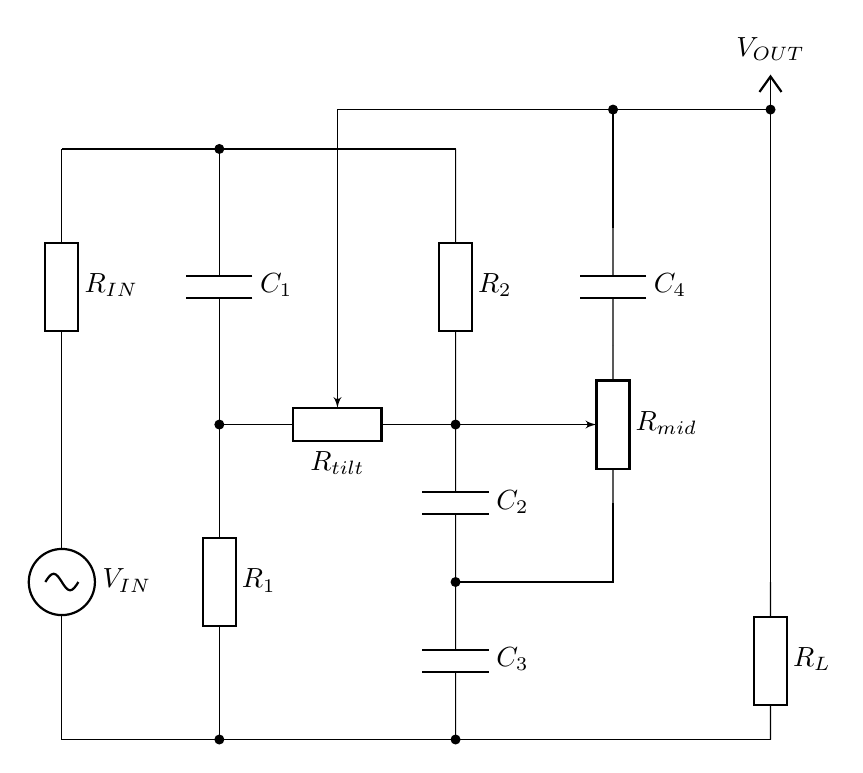
\begin{tikzpicture}
	\draw (2, 6) to[sinusoidal voltage source, l=$V_{IN}$] (2, 2);

	\draw (2, 9.5) to[european resistor, l=$R_{IN}$] (2, 6);
	\draw (4, 6) to[european resistor, l=$R_1$] (4, 2);
	\draw (7, 9.5) to[european resistor, l=$R_2$] (7, 6);
	\draw (11, 4) to[european resistor, l=$R_L$] (11, 2);

	\draw (9, 5) to[european potentiometer, l_=$R_{mid}$] (9, 7);
	\draw (4, 6) to[european potentiometer, l_=$R_{tilt}$] (7, 6);

	\draw (4, 9.5) to[capacitor, l=$C_1$] (4, 6);
	\draw (7, 6) to[capacitor, l=$C_2$] (7, 4);
	\draw (7, 4) to[capacitor, l=$C_3$] (7, 2);
	\draw (9, 8.5) to[capacitor, l=$C_4$] (9, 7);

	\draw (2, 2) -- (11, 2);
	\draw (7, 9.5) -- (2, 9.5);
	\draw (11, 10) -- (5.5, 10) -- (5.5, 6.56);
	\draw (8.44, 6) -- (7, 6);
	\draw (9, 5) -- (9, 4) -| (7, 4);
	\draw (9, 8.5) -- (9, 10);
	\draw (11, 4) -- (11, 10);

	\node[vcc] at (11, 10) {$V_{OUT}$};
	\node[circ] at (11, 10) {};
	\node[circ] at (4, 2) {};
	\node[circ] at (4, 6) {};
	\node[circ] at (4, 9.5) {};
	\node[circ] at (7, 2) {};
	\node[circ] at (7, 4) {};
	\node[circ] at (7, 6) {};
	\node[circ] at (9, 10) {};

\end{tikzpicture}
\end{document}